\documentclass{article}

\usepackage{fancyhdr}
\usepackage{graphicx}
\usepackage{extramarks}
\usepackage{enumerate}
\usepackage{amsmath}

\topmargin=-0.45in
\evensidemargin=0in
\oddsidemargin=0in
\textwidth=6.5in
\textheight=9.0in
\headsep=0.25in

\linespread{1.1}

\pagestyle{fancy}
\lhead{\paperAuthorName}
\chead{\paperTitle}
\rhead{\currentDate}
\lfoot{\teamName}
\renewcommand\headrulewidth{0.4pt}
\renewcommand\footrulewidth{0.4pt}

\setlength\parindent{0pt}

\graphicspath{ {images/} }

\newcommand{\enterSectionHeader}[1]{
\nobreak\extramarks{#1}{#1 continued on next page\ldots}\nobreak
\nobreak\extramarks{#1 (continued)}{#1 continued on next page\ldots}\nobreak
}

\newcommand{\exitSectionHeader}[1]{
\nobreak\extramarks{#1 (continued)}{#1 continued on next page\ldots}\nobreak
\nobreak\extramarks{#1}{}\nobreak
}

\setcounter{secnumdepth}{0}
\newcounter{customSectionCounter}

\newcommand{\customSectionName}{}
\newenvironment{customSection}[1][Section \arabic{customSectionCounter}]{
\stepcounter{customSectionCounter}
\renewcommand{\customSectionName}{#1}
\section{\customSectionName}
\enterSectionHeader{\customSectionName}
}{
\exitSectionHeader{\customSectionName}
}

\newcommand{\infoBox}[1]{
\noindent\framebox[\columnwidth][c]{\begin{minipage}{0.98\columnwidth}#1\end{minipage}}
}

\newcommand{\customSubSectionName}{}
\newenvironment{customSubSection}[1]{
\renewcommand{\customSubSectionName}{#1}
\subsection{\customSubSectionName}
\enterSectionHeader{\customSectionName\ [\customSubSectionName]}
}{
\enterSectionHeader{\customSectionName}
}

\newcommand{\paperTitle}{Address\ Book\ Design\ Document}
\newcommand{\paperAuthorName}{Zachary\ Trudo}
\newcommand{\teamName}{Team\ 666}
\newcommand{\currentDate}{2017-01-17}

% Title Page
\title{
\vspace{2in}
\textmd{\textbf{\paperTitle}}\\
\vspace{3in}
}

\author{\textbf{\paperAuthorName}}
\date{\currentDate}
\begin{document}

\maketitle

\newpage
\tableofcontents
\newpage

\begin{customSection}[Overview]
  Our goal is to create an Address Book meeting the requirements of the product
  specifications provided by Prof. Faulk. We will do this in three main phases:

  \begin{itemize}
    \item Minimum Viable Product (MVP) \\
      This will be the phase where we implement a minimial product that can
      perform the basic CRUD operations of an address book.
    \item GUI Implementation
      This will be the phase where we develop the GUI and link it to our MVP.
    \item Feature implementation
      This is the phase where we implement all features that are not CRUD related.
  \end{itemize}
\end{customSection}

\newpage
\begin{customSection}[Minimum Viable Product (MVP)]
  The minimum viable product will be an command line address book that can perform
  the basic Create, Read, Update, Delete (CRUD) commands for an address book. This
  first step will provide us with a solid platform to link a GUI to in the future.
  \\
  Objects:
  \begin{itemize}
    \item Address \\
      This is the most basic object. Will contain all of the 'standard' address
      parameters, and functions for interacting with them.
      \begin{center}
          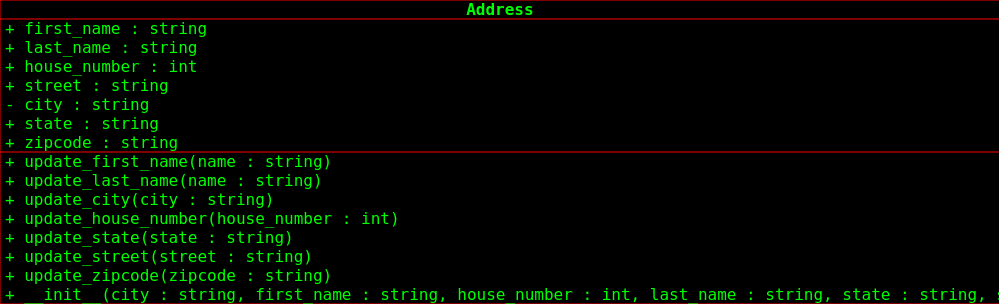
\includegraphics[width=\textwidth]{AddressUML}
      \end{center}
    \item AddressBook\\
      This is the book itself, it will handle updates to the book.
      \begin{center}
          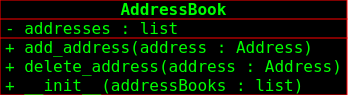
\includegraphics[width=\textwidth]{AddressBookUML}
      \end{center}
    \item FileOps\\
      This will be a static class that has the methods for interaction with the
      file system, producing address books from disk, and saving them to file
      using the YAML format. 
      \begin{center}
          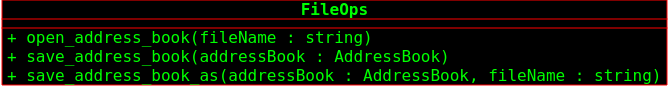
\includegraphics[width=\textwidth]{FileOPSUML}
      \end{center}
      
  \end{itemize}

  
\end{customSection}

  

\end{document}
